\documentclass[12pt]{article}
\usepackage{graphicx}

\textwidth=160mm
\textheight=250mm
\oddsidemargin=0mm
\evensidemargin=0mm
\topmargin = -20mm

\pagestyle{empty}

\begin{document}
\begin{center}
\large Using the MCLURS array  \\[5mm]

\footnotesize John Hallam \\[5mm] 
\today \\[5mm]
\end{center}

\section{Taking Delivery}

\begin{description}
\item[Unpacking.] ~\\

  Each box shipped contains an array Box, a disk Box, 8 cables, 10
  microphones and various extra cables and odds and ends.

  Take out the array Box, open it, and remove the packing material.

  Taped to the inside of the Box there will be a micro-SD card, which
  should be inserted into the appropriate slot on the Raspberry Pi --
  the top circuit board inside the metal box, see
  Figure~\ref{fig:sdcard} below.

\begin{figure}[bh]
  \begin{center}
    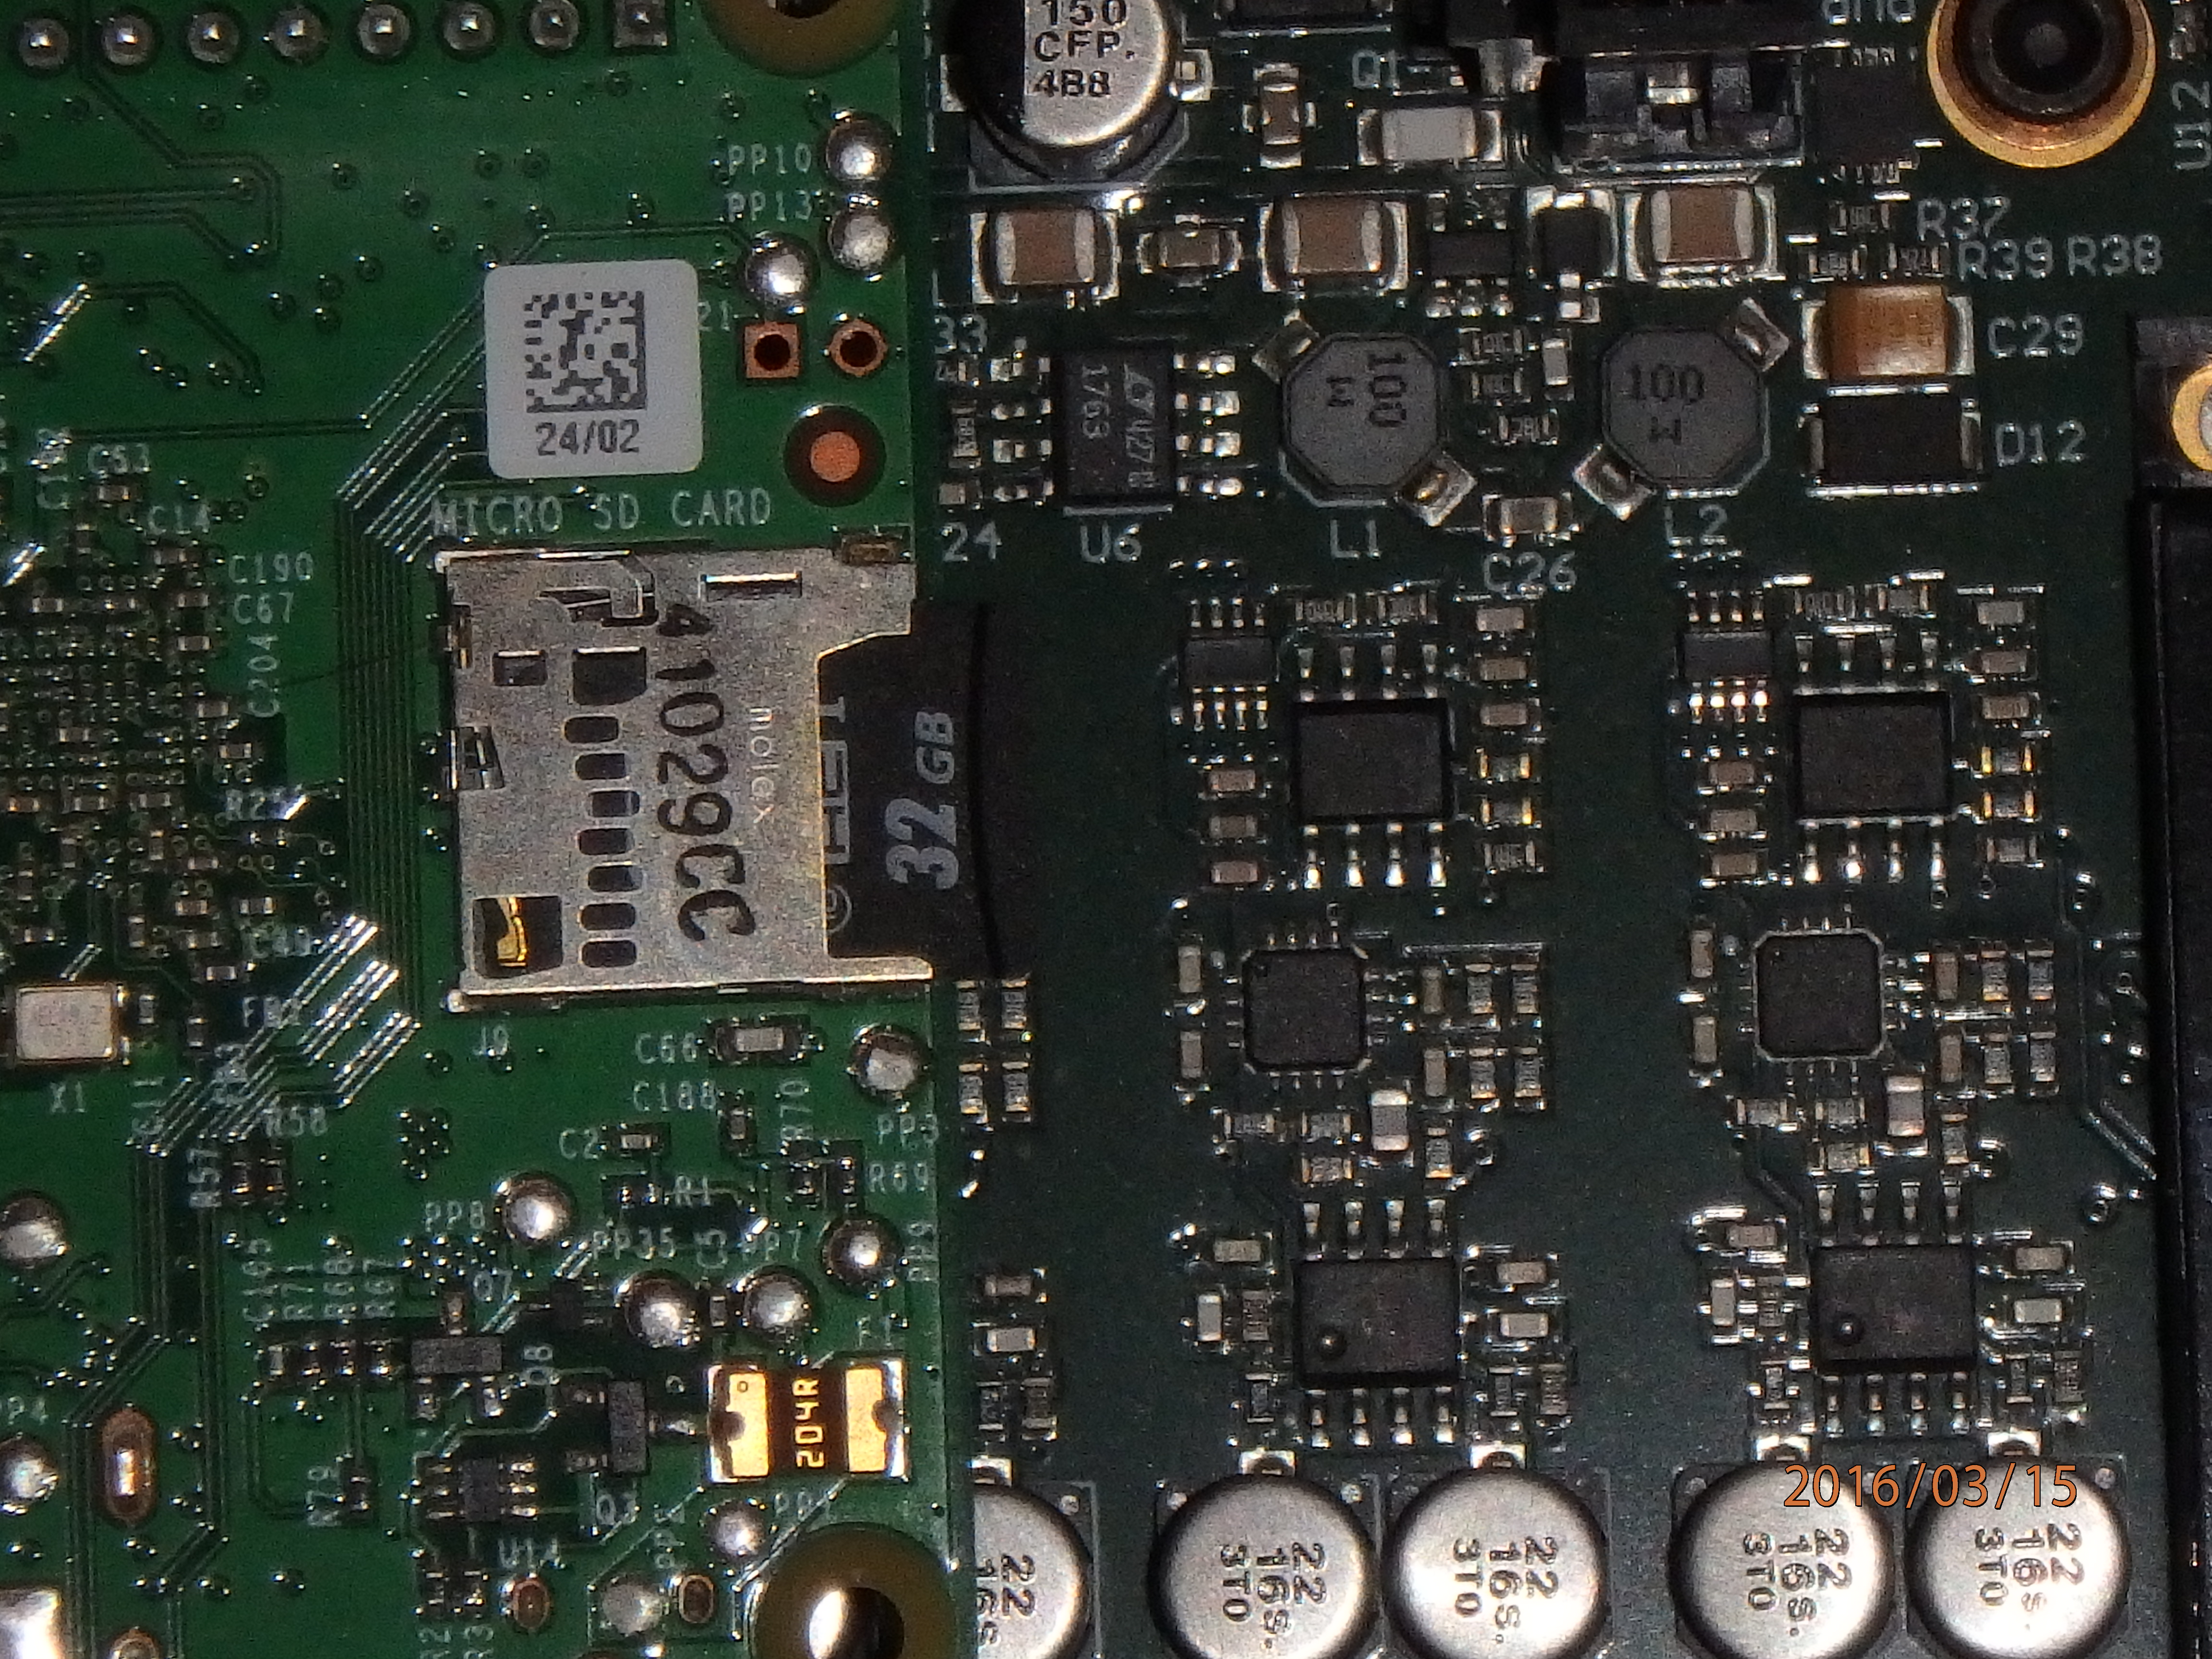
\includegraphics[width=0.9\linewidth]{P3150230}

    \caption{\label{fig:sdcard}
%
      Picture of the electronics inside the Box.  The Channel sockets
      are off the bottom of this image.  On the right is the analog
      card; the edge of the Raspberry Pi (RPi) is in the middle of the
      image and the right end of the RPi is at the left of the image.
      The micro-SD card is inserted into the socket on the RPi board
      in the middle of its right edge, central in the picture -- the
      card in the picture is the black object with ``32 GB'' written
      on it in the metal socket labelled 41029CC.  Your RPi may have a
      different label.}
  \end{center}
\end{figure}

\item[Checking.] ~\\

  Plug the Box together (leaving the lid off initially), that is:

  \begin{enumerate}
  \item  Attach the bench power supply unit to the Box using the power wire

  \item  Turn on the power;  various lights should light up on the circuit boards
       inside the metal box.

  \item  Wait for about 30 seconds

  \item  Attach the Box network cable and plug the other end into your computer
  \end{enumerate}

  At this point, if everything is working fine, your computer should
  soon be given a network address.  You can then talk to the Box using
  PuTTY (see separate instructions for installing PuTTY).

  To test the Box, try to connect to it using PuTTY.  Its name is
  printed on the side of the weatherproof case -- either batpi3 or
  batpi4.  Use the user name \texttt{bbu} and the password
  \texttt{funfunfun} to connect.  If everything is working, you will
  see a black terminal window on your computer with a prompt for input
  (ending in a \texttt{\$} sign).

  Test the Box by typing
\begin{quotation}\texttt
       date[ENTER]
\end{quotation}
  at the prompt.  You should see a line of information on the Box's
  idea of the current date, and a new input prompt.  If that works,
  the basic computing functions of the Box are working fine.

  Now type
\begin{quotation}\texttt
      sudo shutdown -h now[ENTER]
\end{quotation}
  at the prompt.  After a moment the window on your computer will
  close.  Turn off power to the Box and disconnect the cables.

  \item[Finally...] ~\\

  Put a bag of silica gel inside the weatherproof outer box (there is
  a set of silica gel bags with the main cables in one of the shipped
  boxes).

  Fix the weatherproof box lid back on.

\end{description}

\section{Using the Array}

\subsection{Setting Up the Array}

\begin{enumerate}

   \item  Attach microphones to the cables and cables to the Box, as
        many as you wish to use up to the full 8.

   \item  Attach the hard disk to the Box using the special cable.

   \item  Attach the power wire to the Box, either battery or bench
        power unit depending what you want to do.  Turn on the power
        or attach the battery.  The Box will start to boot up.

   \item  Wait for 30 seconds or so

   \item  Attach the network cable to the Box and your computer.  When
        your computer gets a network address, connect to the Box using
        PuTTY.  Log in as the \texttt{bbu} user.  You are now ready to go.

\end{enumerate}

\subsection{Starting the Array}

The array operation is controlled using the \texttt{array} command.

At the input prompt, type
\begin{quotation}\texttt
      array setup[ENTER]
\end{quotation}
After about 30 seconds, the input prompt should return, under a line
of status information saying that the array is ready.

You can now do various things.  For instance, to check what
microphones are connected, type
\begin{quotation}\texttt
      array chan[ENTER]
\end{quotation}
which should give you a list of the connected Channels.  There should
be as many Channels listed as you have microphones connected.  For
each Channel the microphone Name is displayed, as well as the gain and
filter settings.  To change the settings, you can type a command like
\begin{quotation}\texttt
      array gain \textit{n} \textit{gain} \textit{filter}[ENTER]
\end{quotation}
where the things in \textit{italic} stand for values you choose.
\textit{n} can be between 1 and 8, or the word \texttt{all} to affect
all Channels identically.  \textit{gain} can be between 0 (0~dB extra
gain) and 255 (60~dB extra gain). \textit{filter} can be either
\texttt{hp} for high-pass (bat recordings) or \texttt{ap} for all-pass
(e.g. for frog recording).  Examples of the command might be
\begin{quotation}\texttt
      array gain 3 128 hp[ENTER]
\end{quotation}
i.e. set the gain of Channel 3 to 128 (30~dB extra gain) and use the
high-pass filter (cutoff around 16~kHz).
\begin{quotation}\texttt
      array gain all 0 ap[ENTER]
\end{quotation}
i.e. set the gain of all connected Channels to 0 (i.e. 0~dB extra) and
use the all-pass filter (cutoff around 16~Hz).

You can check the parameters by using the \texttt{array chan} command to
display the Channel settings.  Note that if you try to change the gain
on a Channel with no microphone connected the software will complain.

Once you are happy with the settings, it's time to start the capture
system, using the command
\begin{quotation}\texttt
      array start[ENTER]
\end{quotation}
You should get a reply that begins \texttt{OK}.  At this point, the
ADC is capturing samples from the microphones at a sampling rate of
312.5~kHz, but then throwing them away.  It keeps a window of about 8
seconds in memory.

Everything is now ready for data collection.  You can still change the
Channel setup with the \texttt{array gain} command.

When you have finished work, shut the array down using
\begin{quotation}\texttt
      array stop[ENTER]
\end{quotation}
and then do
\begin{quotation}\texttt
      array eject[ENTER]
\end{quotation}
to release the hard disk.  If you have finished work with the Box, you
can then do
\begin{quotation}\texttt
      sudo shutdown -h now[ENTER]
\end{quotation}
to turn the Box off, and once the window on your computer closes you
can remove the power to the Box.  (Actually, it shouldn't hurt if you
just pull the plug out, but a controlled shutdown is more friendly.)

\subsection{Capturing Data}

Once the array is started, you can use it to take snapshots.  For this
you use the \texttt{trig} command, which is separate from
\texttt{array}.  Set up and start the array as described above.  You
should have an input prompt in the window on your computer where you
talk to the Box.

To take a single snapshot, type in the command:
\begin{quotation}\texttt
      trig -s tcp://127.0.0.1:2468 "my first snapshot"[ENTER]
\end{quotation}
including the quotation marks.  The snapshot is taken when you hit
[ENTER] and it consists of 1500~milliseconds of recorded data, of
which 1000~milliseconds are before you hit the trigger (pressed
[ENTER]) and~500 after after that moment.  The snapshot will be called
"my first snapshot".

To check whether everything worked, you can use the command
\begin{quotation}\texttt
      array snap[ENTER]
\end{quotation}
which will give you a (rather cryptic) list of completed snapshots
from this session.  In general, if \texttt{trig} finished silently the snapshot
request was accepted by the system; if there was an immediate problem
you will see a reply from \texttt{trig} beginning \texttt{NO:}.  On the other
hand, if a problem arises with an accepted snapshot request, the
\texttt{array snap} command will show that.  But this should be
uncommon.

\texttt{trig} is actually a very versatile command.  For example, you
can change the pre- and post-trigger times in your request by
providing a \texttt{--pre} and \texttt{--pst} argument when you give
the command.  For instance
\begin{quotation}\texttt
      trig -s tcp://127.0.0.1:2468 --pre 5000 "my next snapshot"[ENTER]

      trig -s tcp://127.0.0.1:2468 --pre 5000 --pst 2500 "my big snapshot"[ENTER]

      trig -s tcp://127.0.0.1:2468 --pre 50 --pst 7500 "my last snapshot"[ENTER]
\end{quotation}
will request respectively a snapshot with 5000~ms of data from before
the trigger point and 500~ms from after; a snapshot with 5000~ms
before and 2500~ms after the trigger; and a snapshot with 50~ms before
and 7.5~seconds after the trigger.  The biggest snapshot you can take
with \texttt{trig} is about 8~seconds long in total.

You can also ask \texttt{trig} to name your snapshots for you.  There are
various options but the simplest is to have them called
\texttt{snap000000}, \texttt{snap000001}, and so on.  For this, you
have to ask \texttt{trig} to make multiple snapshot requests.  As an example,
suppose you want to take a set of snapshots for an experiment, each of
them 4 seconds long with 3 seconds before the trigger point, named
automatically, you could type:
\begin{quotation}\texttt
      trig -r -s tcp://127.0.0.1:2468 --pre 3000 --pst 1000 --auto=seq[ENTER]
\end{quotation}
Notice the \texttt{-r} (repeat), which tells \texttt{trig} not to stop after one
snapshot request.  When this command is run you will see a different
input prompt: one from \texttt{trig}.  Each time you hit [ENTER], a
new snapshot request is sent to the array software using the next name
in the sequence \texttt{snap000000} and so on.  To stop taking
snapshots, type
\begin{quotation}\texttt
      q[ENTER]
\end{quotation}
at the prompt, and \texttt{trig} will finish.  If any snapshot requests are
rejected, you will see a \texttt{NO:} reply after you pressed [ENTER]
for the rejected snapshot; otherwise, you just get a new prompt.  As usual,
\texttt{array snap} will give you a status line for each snapshot.

\subsection{Collecting the Data}

When you have taken some snapshots, you need to get the data out of
the Box.  The simplest way to do this is to shut the Box down, unplug
the hard disk and connect the disk to your computer.  There is a
special USB cable for doing this included in the set of cables.

As stored on the hard disk, a snapshot is currently organised as
follows.  Each snapshot is stored in a folder with a unique name that
will look something like
\begin{quotation}\texttt
   	574c9e64-e131-11e5-adb9-1867b0c03033
\end{quotation}
-- this is done to avoid name clashes when capturing data.  In that
folder are two files called \texttt{metadata} and \texttt{vars.sh} and
a folder called \texttt{samples}.  In the latter folder is a file of
data in S16 format.  The \texttt{metadata} file contains a list of
metadata giving the sampling frequency, the connected Channel
parameters, the Box information, and so on, as well as the name you
gave the snapshot (on the line NAME=...).  Notepad can read the
\texttt{metadata} file, which is just plain text (if you can persuade
your computer to believe it).

The S16 file consists of the samples that were captured from the ADC,
organised in sets of 8, each sample being a 16 bit signed value.
MATLAB, for example, can read such files.

We are working on a \texttt{pack} command that will allow you to turn
this structure into something more usable, for instance a WAV file
with the metadata included.

\end{document}

